%   preamble {{{1  %
%%%%%%%%%%%%%%%%%%%%

\documentclass[notes=show]{beamer}

\usepackage[utf8]{inputenc}
\usepackage[english]{babel}

%  beamer theme {{{1  %
%%%%%%%%%%%%%%%%%%%%%%%

\usetheme{metropolis}           % Use metropolis theme
\metroset{background=light}
\setbeamertemplate{frame footer}{

\includegraphics[width=1cm, keepaspectratio]{images/max_planck.png}
} %Metropolis defined
\setbeamercolor{background canvas}{bg=white}



\title[Ab initio studies \ldots]{
  
\includegraphics[width=2cm, keepaspectratio]{images/max_planck.png}
 \hfill
  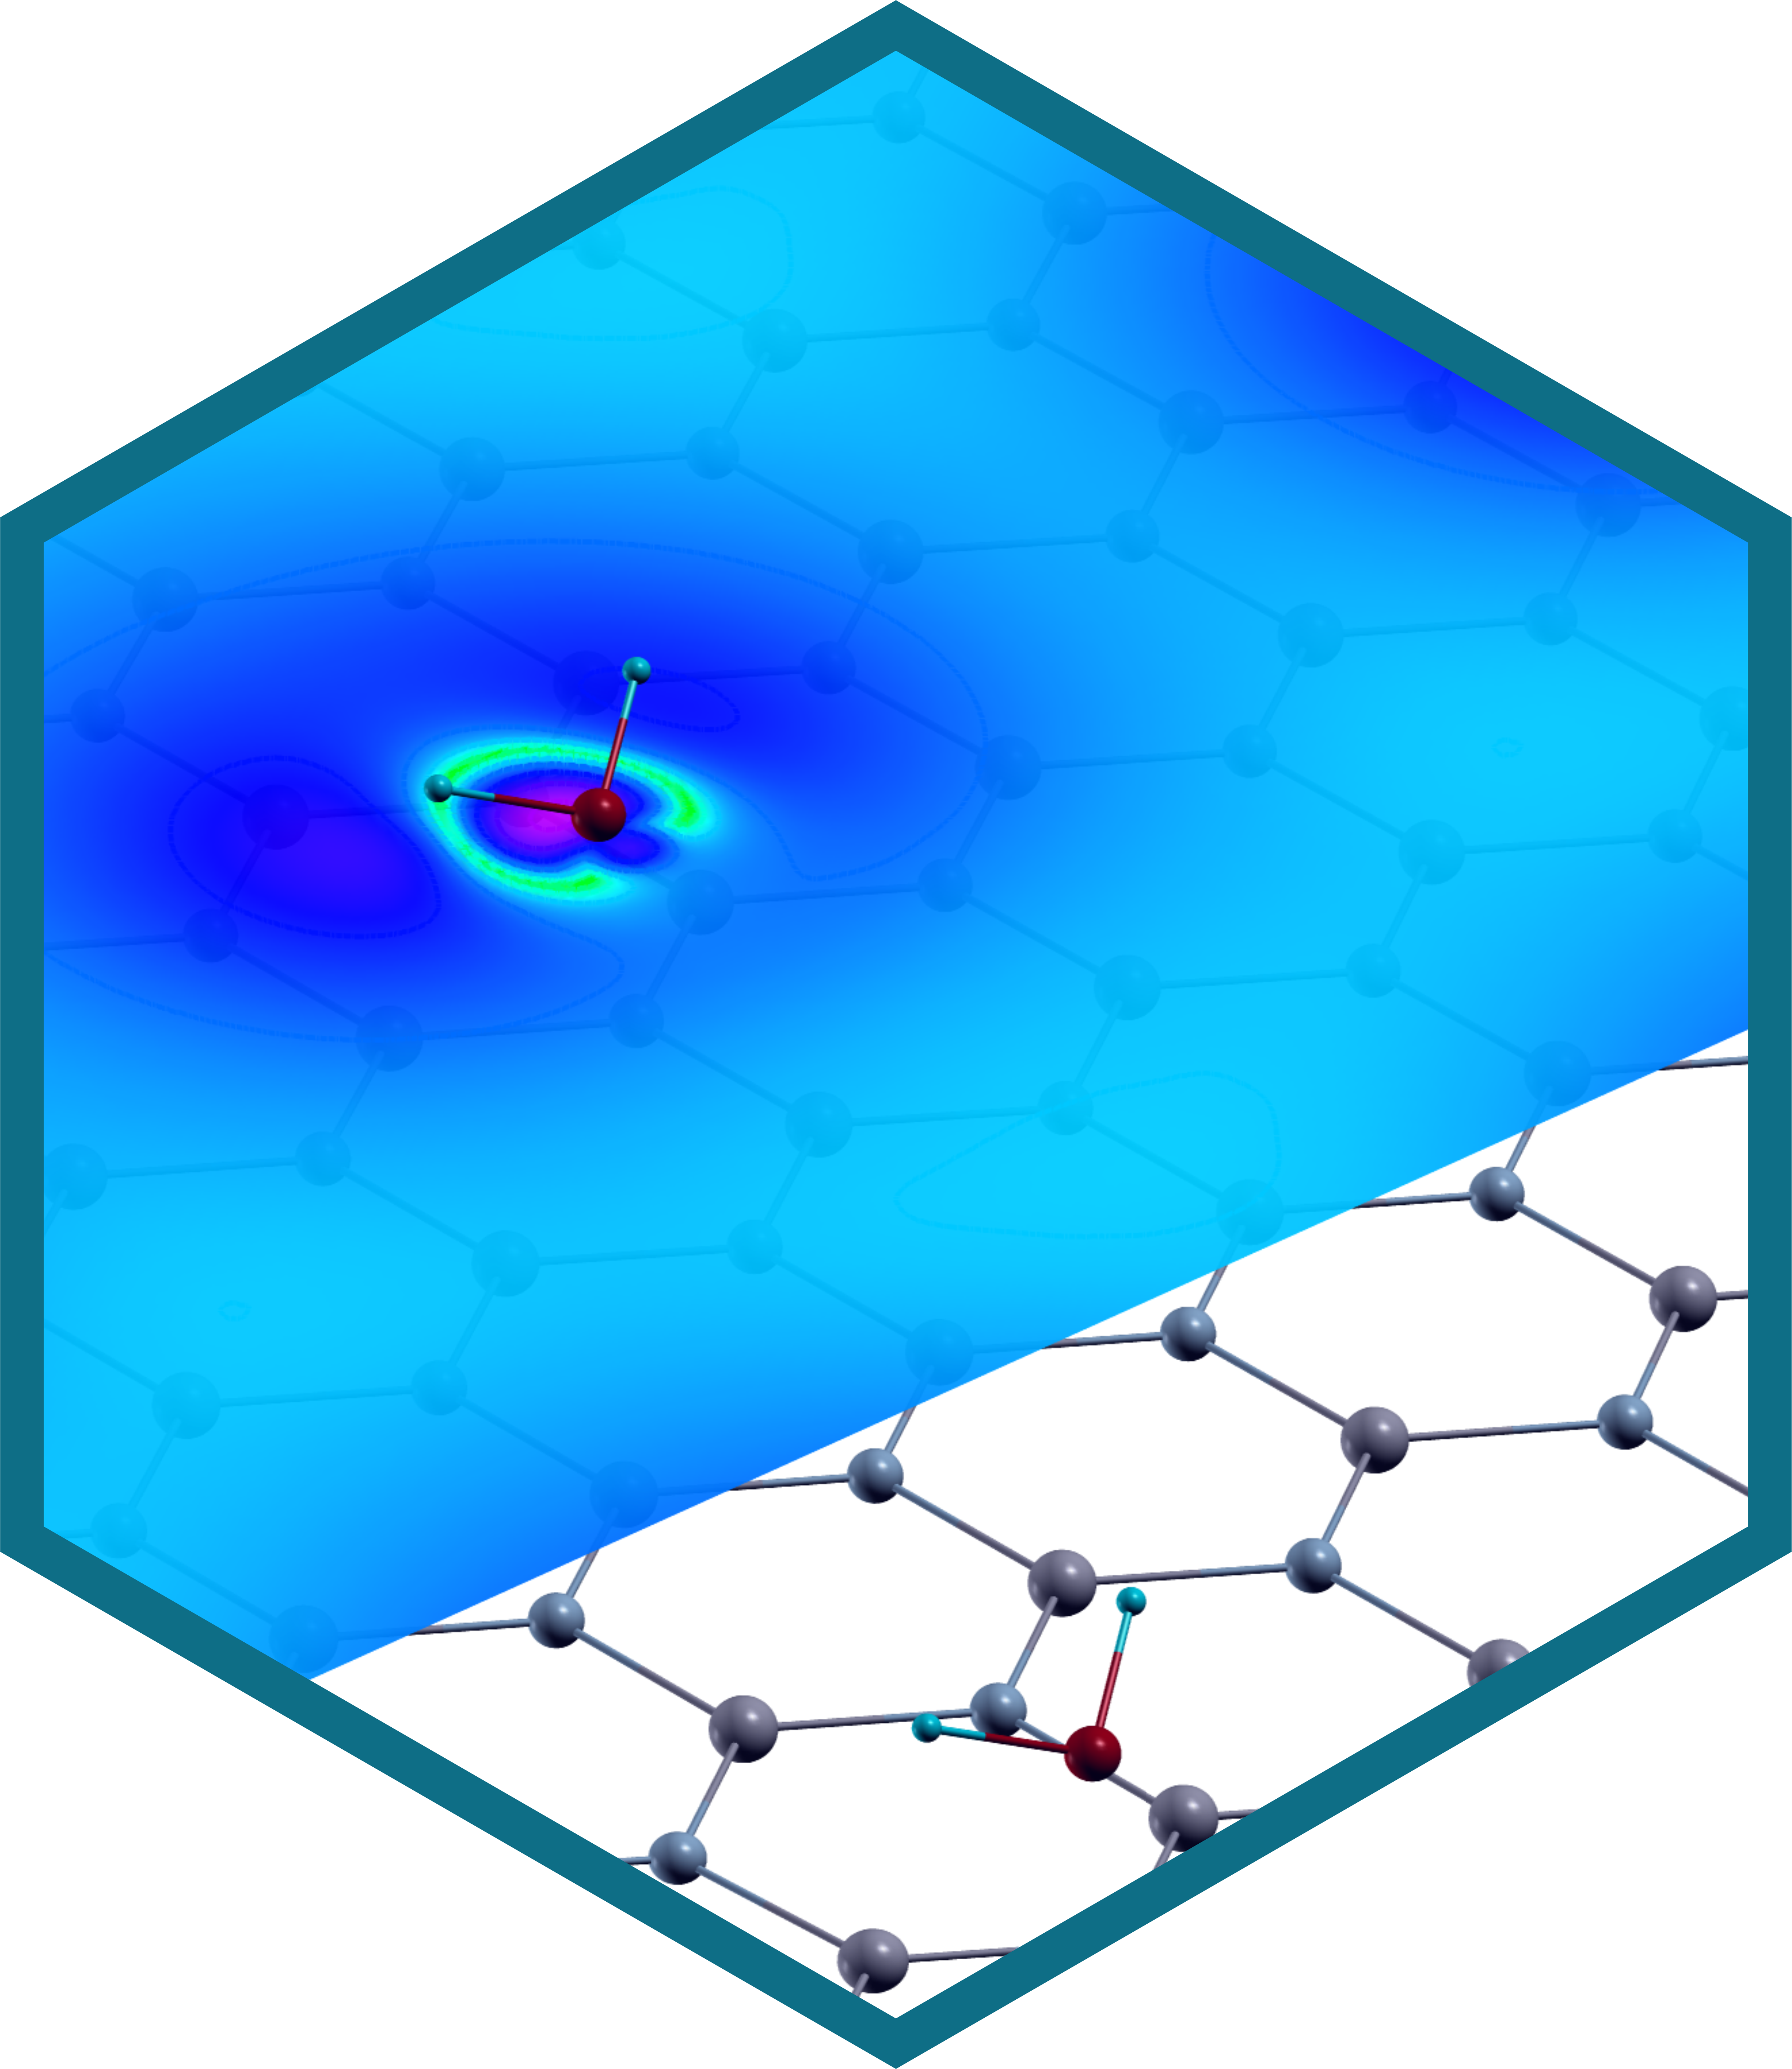
\includegraphics[width=1.4cm, keepaspectratio]{images/logo_andreas.png} \\
  Ab initio studies of vacancy-impurity complexes in cubic and hexagonal
  diamond
}
\date{July 29, 2016}


\author{Alejandro Agustí Martínez-Soria Gallo}
\institute{
  Max-Planck Institute for solid state research\\
  \textbf{Advisor}: Dr. Andreas G\"uneis
}


\begin{document}


%  title {{{1  %
%%%%%%%%%%%%%%%%

\maketitle

\note{

  Hello my name is Alejandro and I am currently working on my master
  thesis project entitled:\\ \textit{Ab initio studies of
  vacancy-impurity complexes in cubic and hexagonal diamond}\\ The
  supervision of the project is conducted by Dr. Andreas Grueneis , head
  of group at the MPI for solid state research. We engaged in this
  project as a joint collaboration with the third physical institute of
  this University, which is led by Prof. Joerg Wrachtrup.

}

\begin{frame}{Contents}
\tableofcontents

\note{

  In the following we will provide some basic background
  in the field of vacancy-impurity complexes and
  we will quickly introduce some of the techniques used
  to model and calculate their electronic properties.

  The main systems of this work will be introduced
  and we will finish by giving a quick outlook into
  the possible future directions that this research could
  be led into.

}

\end{frame}




\section{Aim and scope of the work} %{{{1
\begin{frame}{Aims and motivation}
  \begin{itemize}

    \item
      Exploration of defect centres using state-of-the-art ab-initio
      theories.

    \item
      Benchmark ab initio theories with well-known
      experimental data.

    \item
      Systematic characterisation of defect fingerprints: ZFS, ZPL.

    \item
      Search for new defects with tailored properties.


  \end{itemize}

  \begin{columns}
    \begin{column}{0.5\textwidth}
  \begin{center}
    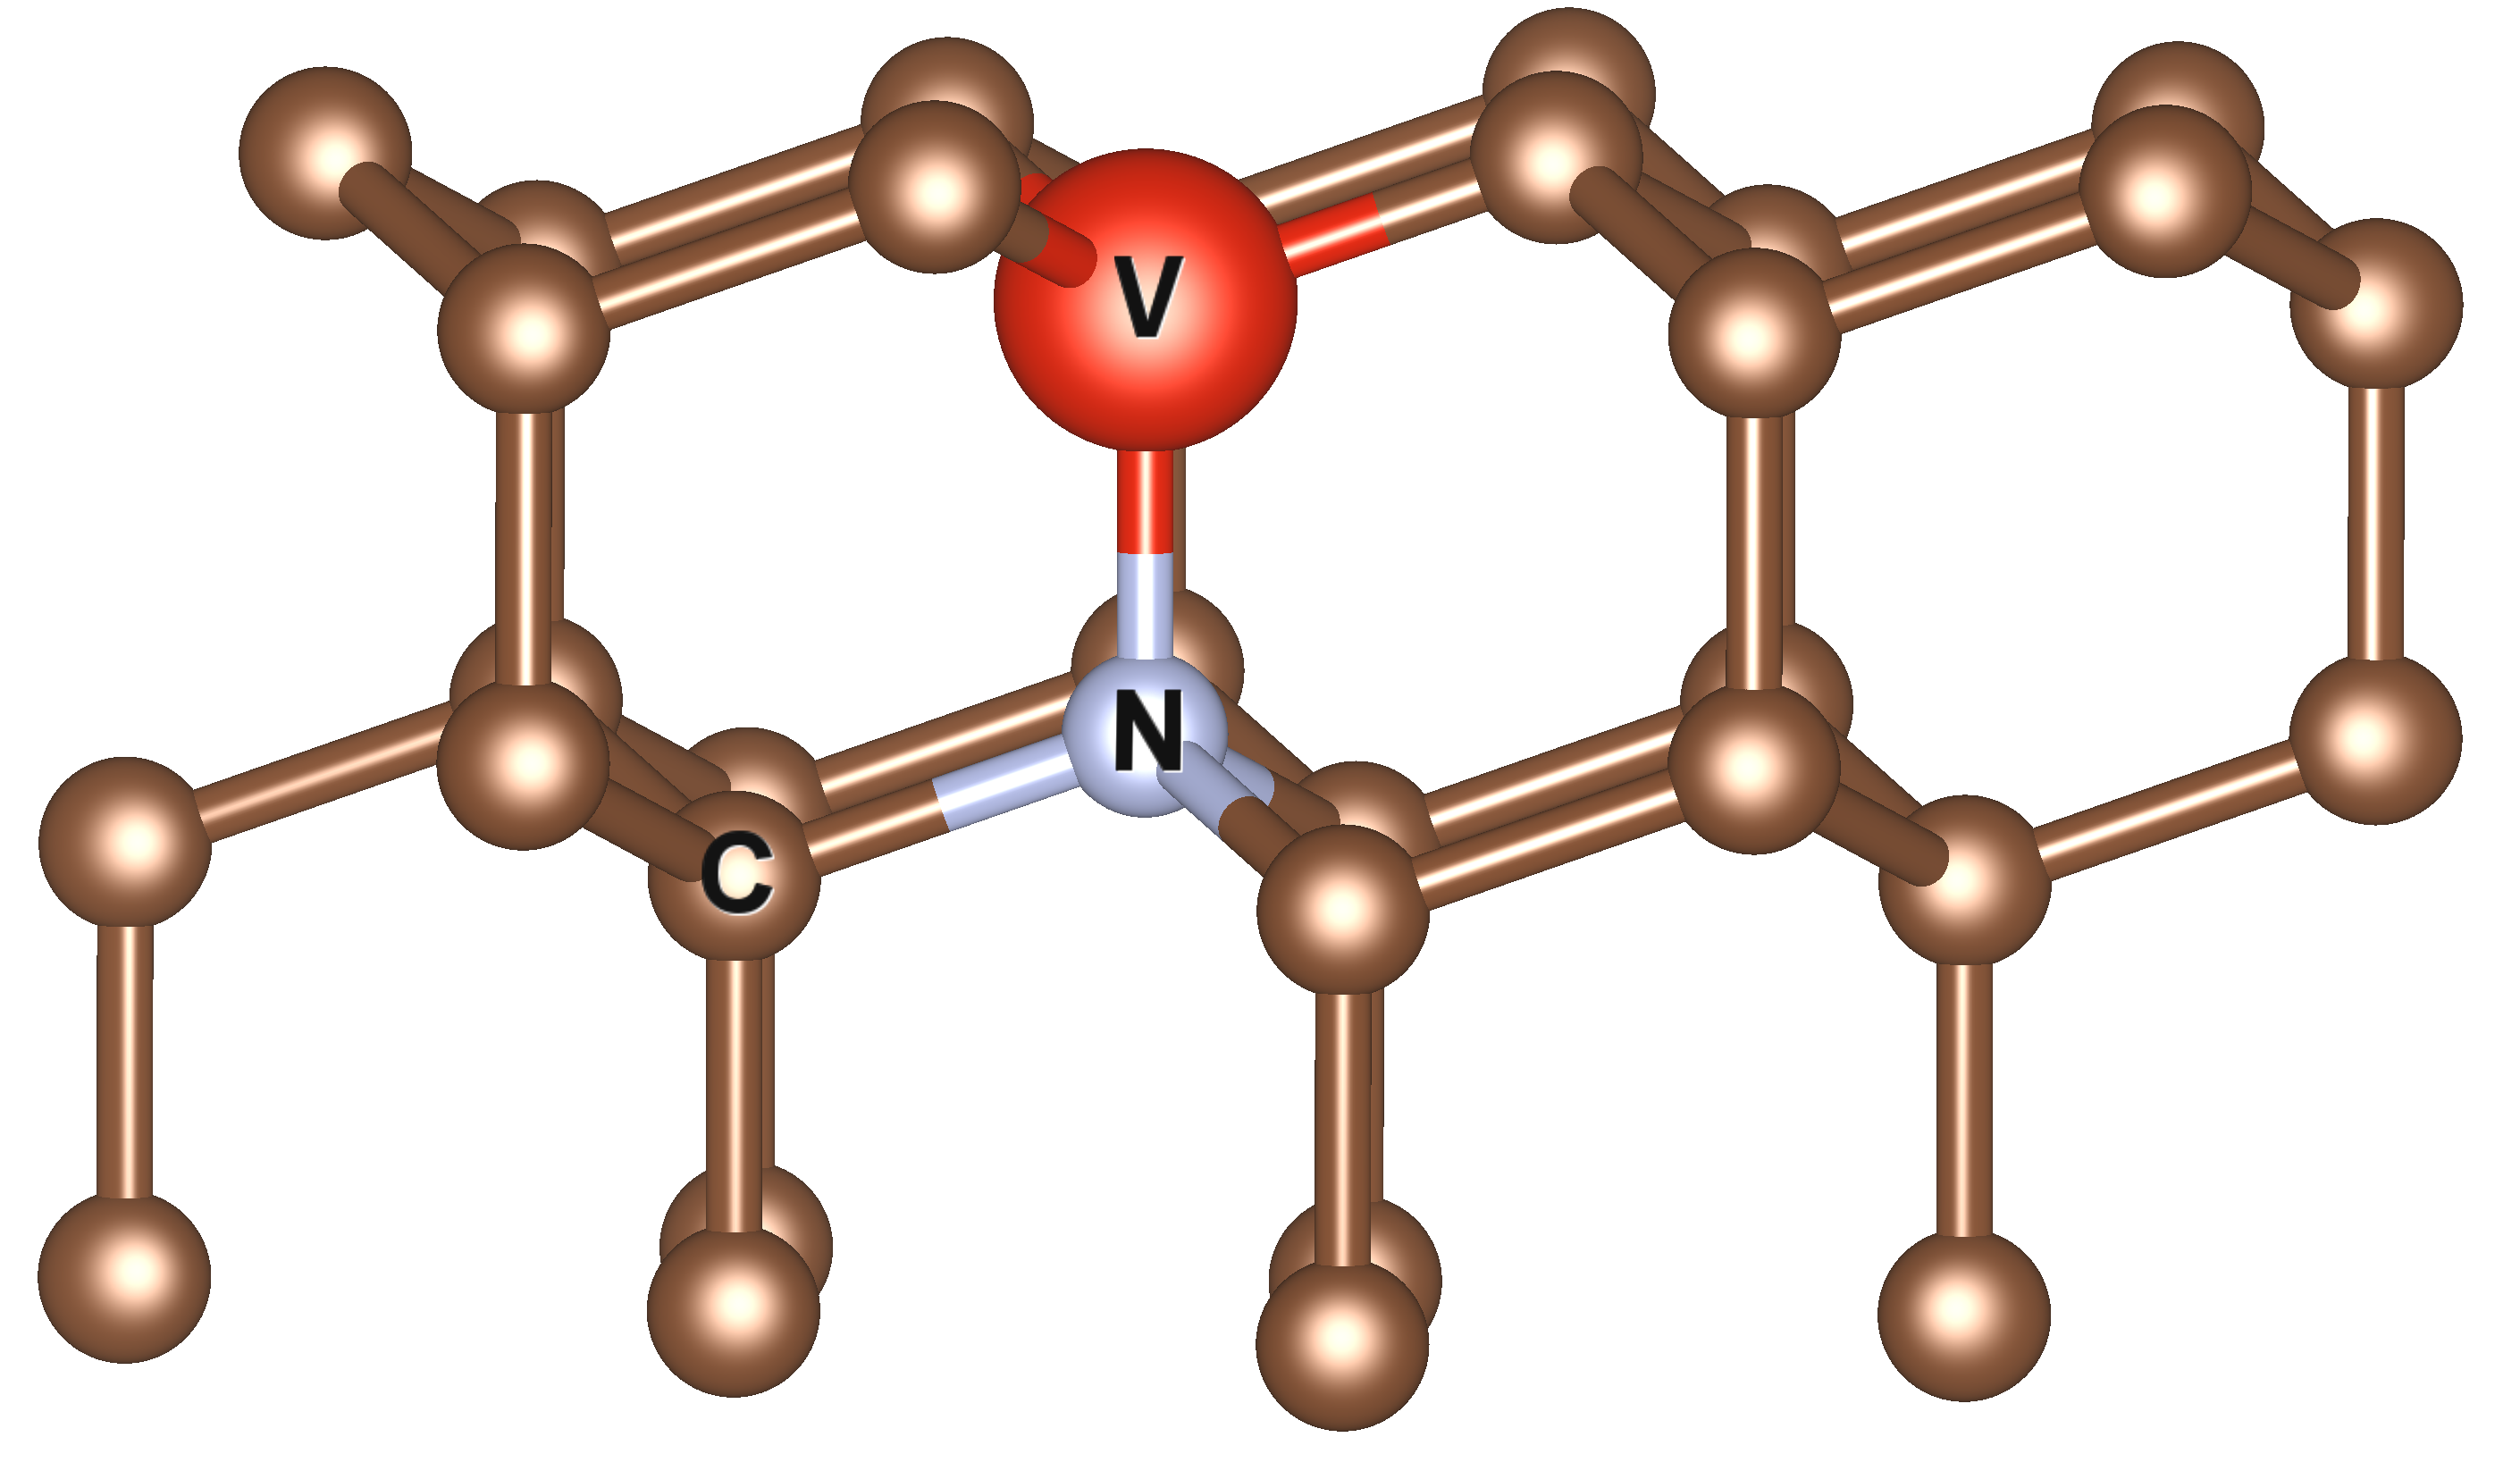
\includegraphics[width=1\textwidth]{images/POSCAR_16_view.png}
  \end{center}
    \end{column}
    \begin{column}{0.5\textwidth}

    \end{column}
  \end{columns}

  \note{

    So the main aim of this work is to computationally
    treat electronic properties of defect centers in diamond
    using state-of-the-art ab initio theories.

    Through this exploration we hope to recover many well-known
    experimentally verified quantities.

    In order to do this we use several purely theoretical
    results to orient our calculations into the right direction.
    (e.g. Markus' Gruppentheorierechnungen)

  }

\end{frame}


\section{Introduction} %{{{1


\begin{frame}{Nitrogen Vacancy Centre in diamond (NV center)}
  \begin{center}
    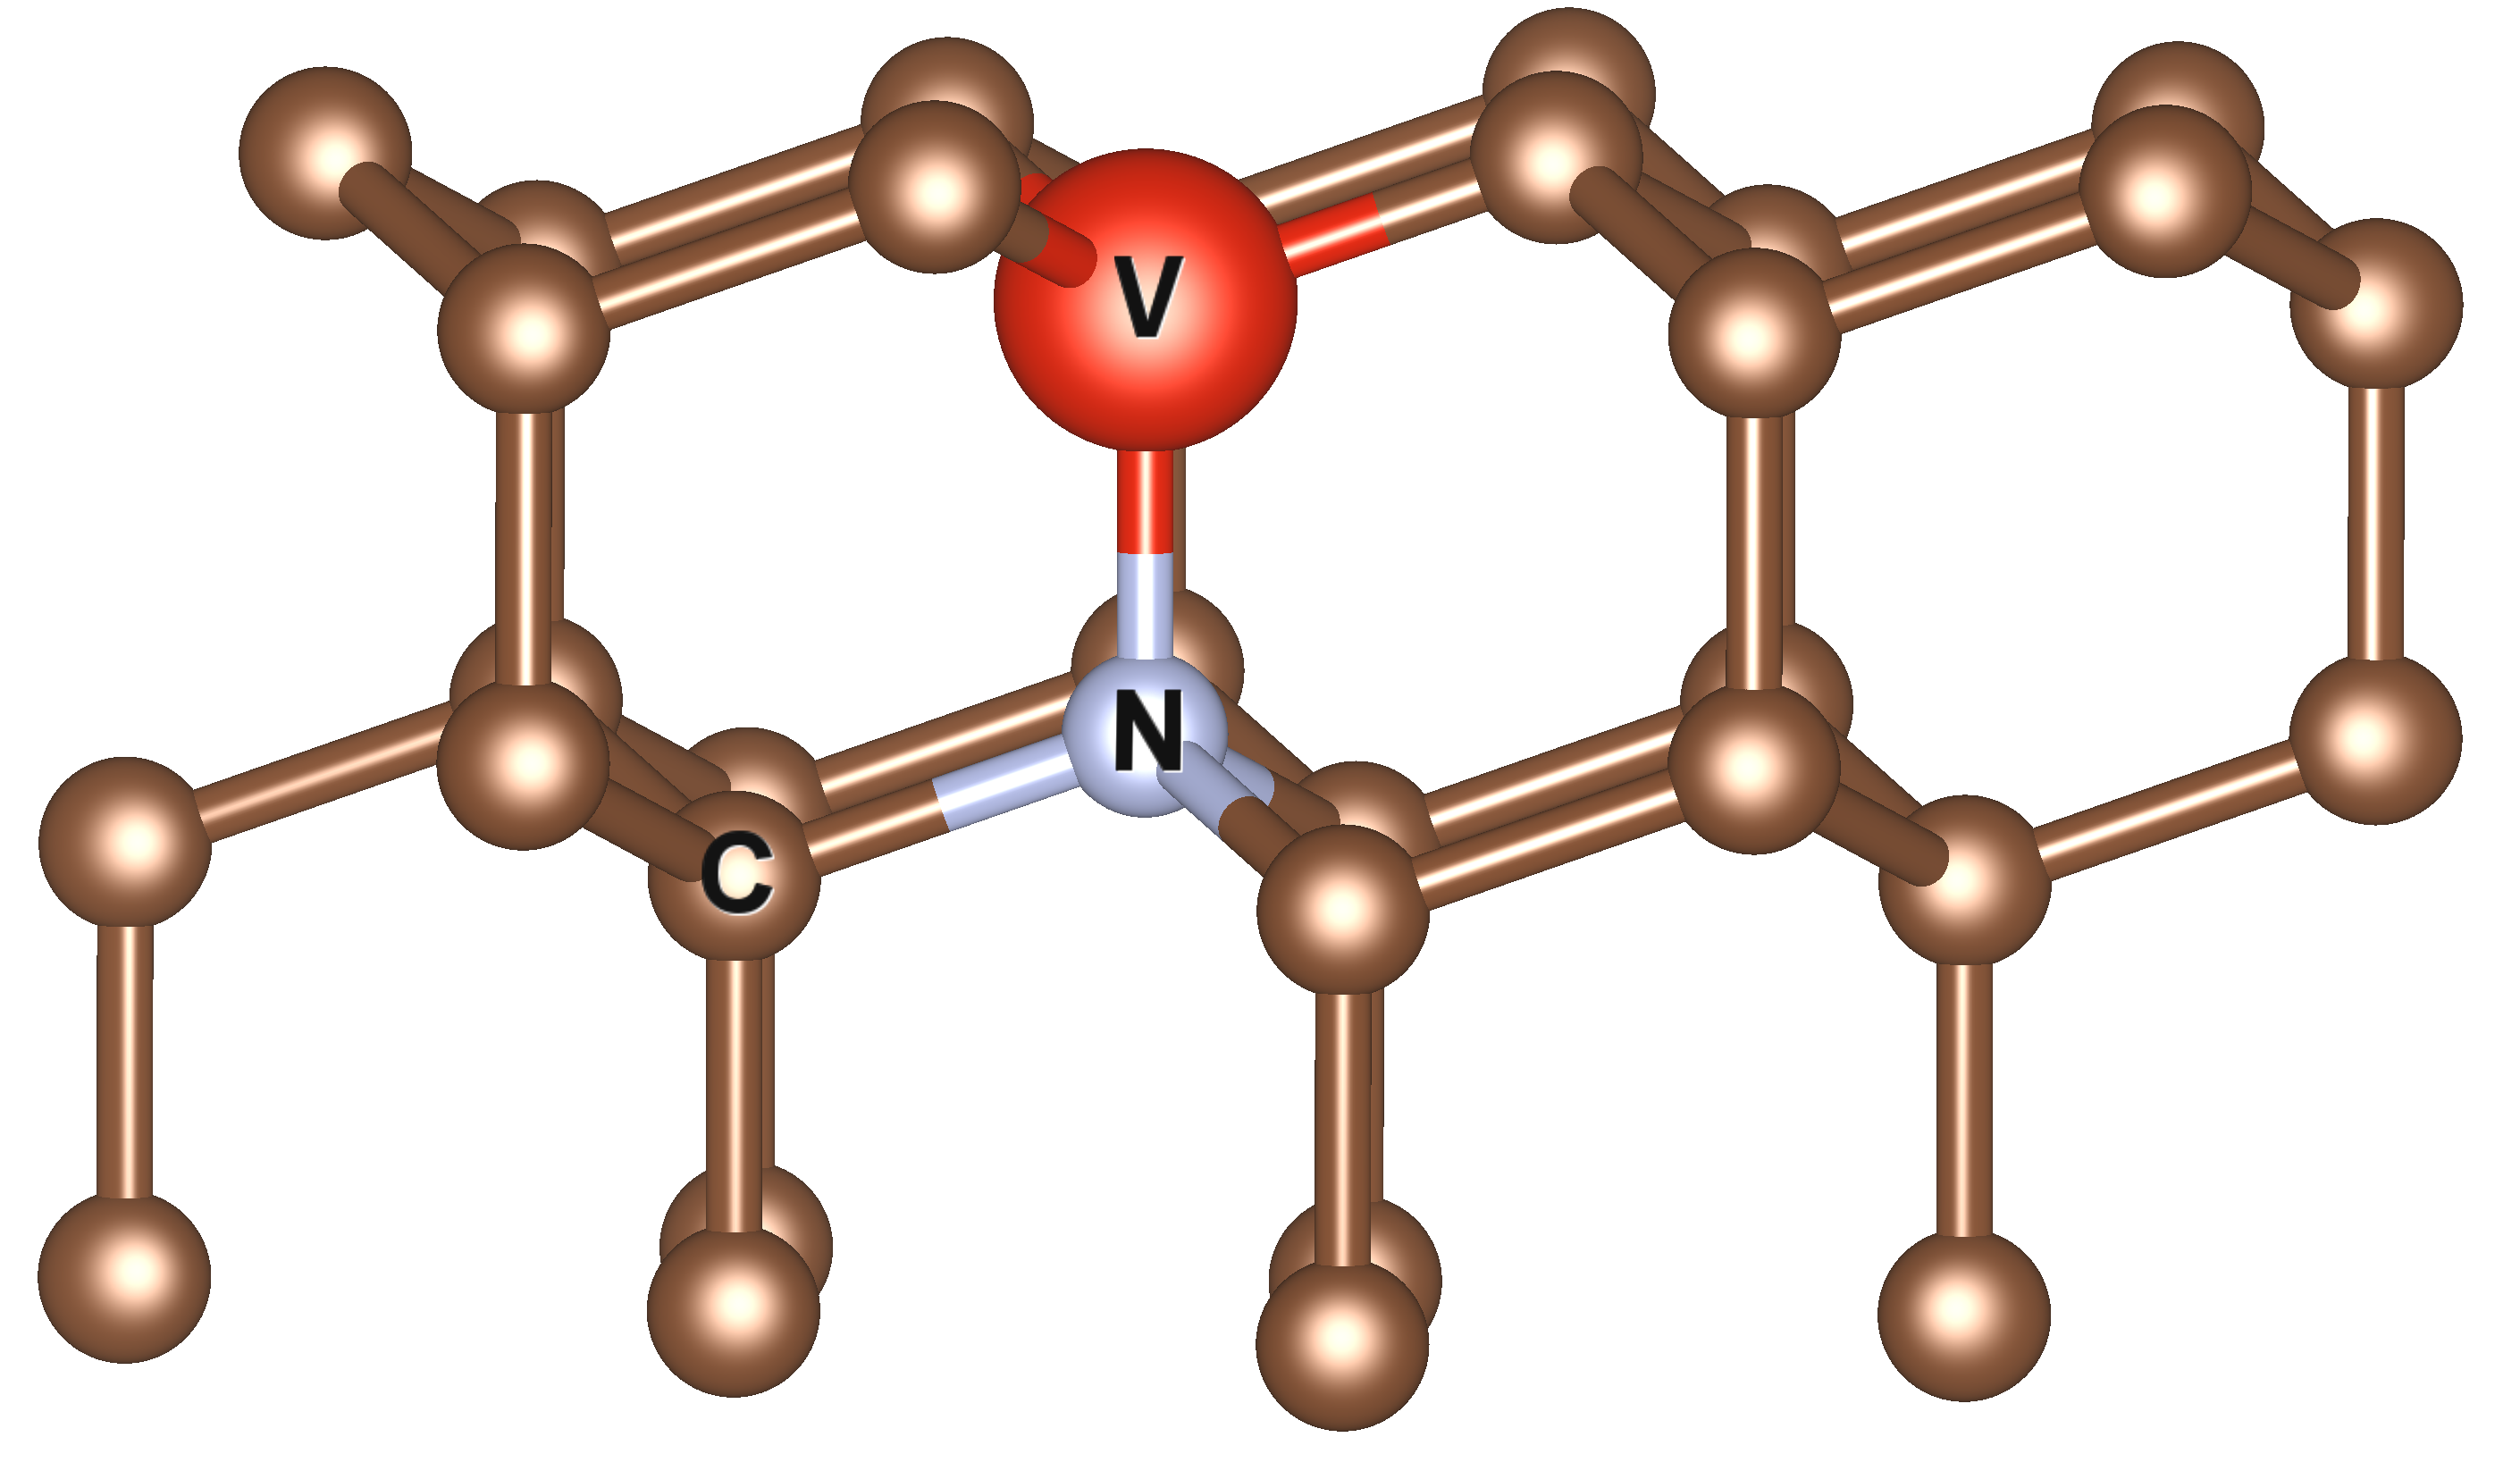
\includegraphics[width=0.9\textwidth]{images/POSCAR_16_view.png}
  \end{center}

  \note{

    So let us just begin by firstly introducing the main actor in this story.
    This is the Nitrogen vacancy impurity center in diamond, as most of you may
    already know.  The big red region is a vacant carbon site and next to it
    lies a nitrogen atom.

    This kind of defects has been researched now for almost 50 years.  However
    it was not until the late nineties when single negatively charged NV
    centres where found. This enabled the demonstration of photo stable single
    photon emitters, which is of course of huge importance for quantum optics.

    The most notable and studied of the NV centers is the negatively charged
    one.

  }

\end{frame}

\begin{frame}{Main level overview: $ \mathsf{NV}^{-} $ }
  \begin{center}
    \includegraphics[width=0.9\textwidth]{images/basic_levels.pdf}
  \end{center}

  \note{

    To explain fluorescence experiments it is essential to have a picture of
    the electronic and vibronic states of a defected diamond sample.
    Theoretical models using a \textit{Linear combination of atomic orbitals}
    (LCAO) give rise to a good prediction of the Spin multiplicity and triplet
    energy levels of the negative NV center.

    From the interplay of theory and experiments arises this electronic level
    scheme. On the one hand we encounter two stable triplet levels, where one
    of them is the ground state of the defect. Between them lie two metastable
    singlet states, which will play an essential role for applications of the
    defect levels.

  }

\end{frame}

\begin{frame}{Triplets overview: $ \mathsf{NV}^{-} $ }
  \begin{center}
    \begin{columns}
      \begin{column}{0.5\textwidth}
        \centering
        \includegraphics[height=.8\textheight]{images/basic_levels_triplets.pdf}
      \end{column}
      \begin{column}{0.5\textwidth}
        \centering
        \includegraphics[height=1\textheight]{images/basic_triplet_configuration.pdf}
      \end{column}
    \end{columns}
  \end{center}

  \note{

    If you have never heard of this defect before, you might be wondering how
    exactly the electrons in the solid body come into play.  In the one
    particle picture of the problem it turns out that we can characterise very
    well these levels by the occupation of the valence states in the body.

    In this picture we can associate to every state with an occupation of the
    topmost states. From this picture we can see that the total spin is one and
    the excitation happens through the promotion of one electron in the level $
    a_{1} $ into one of the degenerated $ e $ levels. This without incurring in
    a spin flip process.

    This we should also find in our calculations.

  }

\end{frame}

\begin{frame}{Zero Field Splitting (ZFS)}
  \begin{center}
    \includegraphics[width=0.9\textwidth]{images/splitting.pdf}\\
    \textbf{\color{red} REVISE E AND D}
  \end{center}

  \note{

    Another important aim of our project is to calculate
    correctly the zero field splitting of the energy levels.

    In this case we are interested in the splitting that
    arises from the Spin-Spin interaction of the electrons.
    This splits into up to three levels the triplet state.
    This splitting is characterised by two parameters,
    $ E $  and $ D $.

    The splitting also arises through strain of the material
    and Zeeman splitting.


  }

\end{frame}

\begin{frame}{Transitions overview: $ \mathsf{NV}^{-} $ }
  \begin{center}
    \includegraphics[width=0.9\textwidth]{images/NV_minus_transitions.pdf}
  \end{center}

  \note{

  One of the main uses that these levels have in common applications of
  the NV center is best understood by the following diagram. In it we
  see the triplets on the left with a splitting in place and the singlet
  states on the right.

  To understand this diagram imagine that the level population
  of the $ m_{s} = 0 $ in the $ ^3A_{2} $ state is much higher
  than the $ x,y $ split states of the same state.
  If we radiate with the right frequency of the energy difference
  between both triplet states, then a non radiative transition
  brings the system into the singlet state, where a radiative
  transition happens. In both possible cases, radiation is produced,
  therefore a detector would take a hold of this radiation.

  If the whole population is however in the upper $ x,y $ states,
  when radiating, since the non radiative transition to the singlet
  states is strong, less radiation will be produced and the detector
  will identify the signal as being darker.

  }

\end{frame}


\begin{frame}{Zero phonon line (ZPL)}
  \begin{columns}
    \begin{column}{0.5\textwidth}
      \includegraphics[width=0.8\textwidth]{images/basic_levels_triplets.pdf}
    \end{column}
    \begin{column}{0.5\textwidth}
      \includegraphics[width=1\textwidth]{images/vibronic.pdf}
    \end{column}
  \end{columns}

  \note{

  To interpret quantitatively some experiments the previous
  picture falls short in some regards.

  Every electronic state is dependent on the ionic constellation.
  This gives rise to the so-called vibronic states.
  For example the ground state has associated with it a given
  ionic constellation. Through excitation to the upper lying
  triplet state since the dynamic of the electrons is much
  faster than the ionic one, the constellation first stays
  static and then relaxes because the potential landscape
  changed due to the difference in the electronic density.

  This gives rise to two different excited states, which
  must be considered in order to reproduce experimental data.

  A very important quantity in this respect is the so-called
  zero phonon line, which as its name indicates characterises
  the transition of the ground relaxed state to the higher
  relaxed state.

  }

\end{frame}

\begin{frame}{Density functional theory (DFT)}
  \textit{``$ \it \Psi  $  contains too much information''}
  \hfill \textit{- Popular saying}
  \begin{itemize}
    \item In principle, DFT delivers the \textbf{exact ground state}.
    %\item The exact electronic ground state of a system is only dependent on
      %the electronic density $ \rho $ .

    \item All quantities are written in terms of $ \rho $ (functional formalism).
    \item E.g.:
      \[
        E[ \rho ] =
        T_{s} [ \rho  ]
        +
        \int  V ( \mathbf{r} ) \rho ( \mathbf{r} ) \ \mathrm{d} \mathbf{r}
        +
        \frac{1}{4\pi \epsilon _{0}}
        \int
        \frac{\rho ( \mathbf{r} ) \rho ( \mathbf{r}' )}{| \mathbf{r} - \mathbf{r}'|}
        \ \mathrm{d} \mathbf{r}\mathrm{d} \mathbf{r}'
        +
        E^{ \mathrm{exact}}_{ \mathrm{xc}} [ \rho ]
      \]
      The exchange correlation potential
      $ E^{ \mathrm{exact}}_{ \mathrm{xc}} [ \rho ] $
      determines the DFT \textit{flavor}.
      In many calculations we use the so-called \textbf{PBE} \textit{(Perdew-Burke-Ernzerhof)} functional.
  \end{itemize}
\end{frame}




\section{Hexagonal diamond and defects} %{{{1


\begin{frame}{Hexagonal diamond}
  \begin{center}
    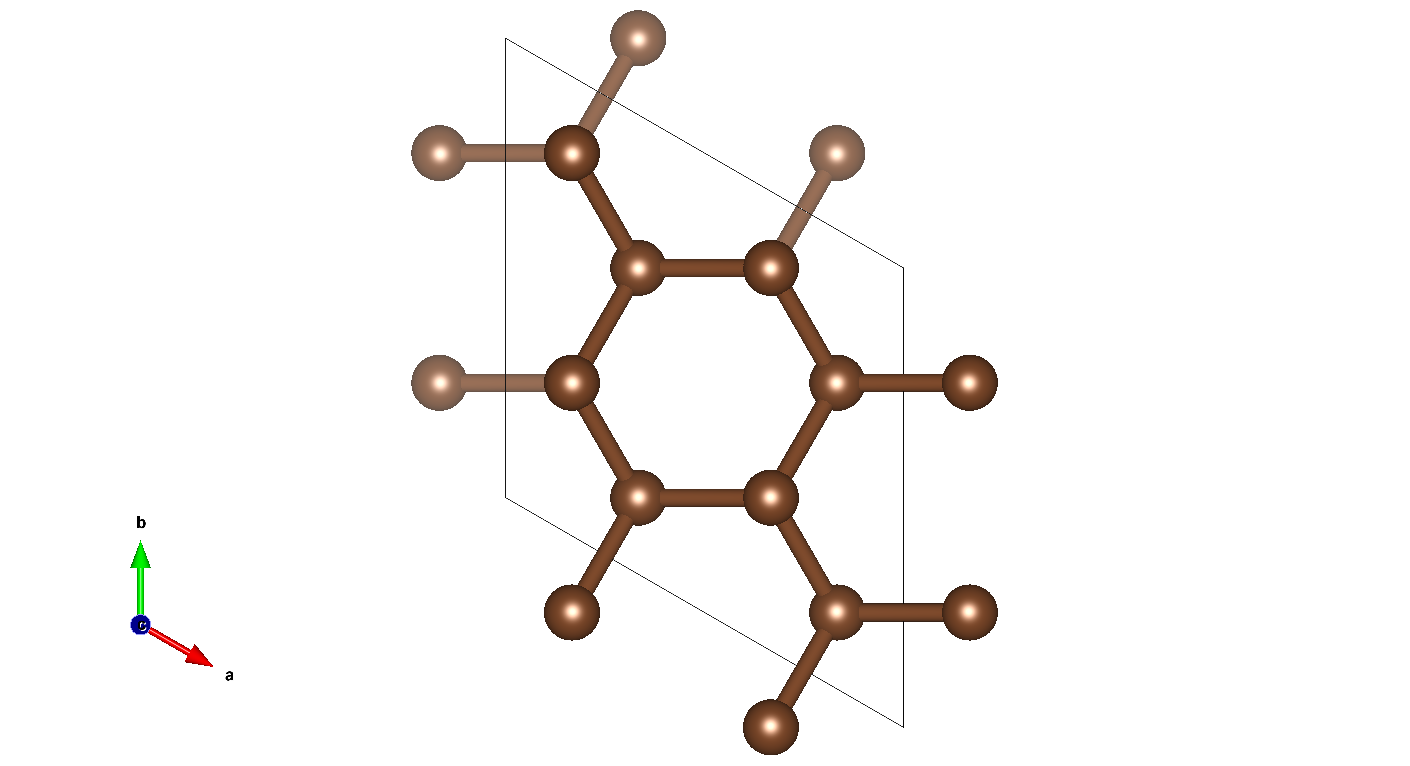
\includegraphics[width=0.5\textwidth, trim=0 0 30em 0,clip]{images/poscar_hex_16_hex-view.png}\\
    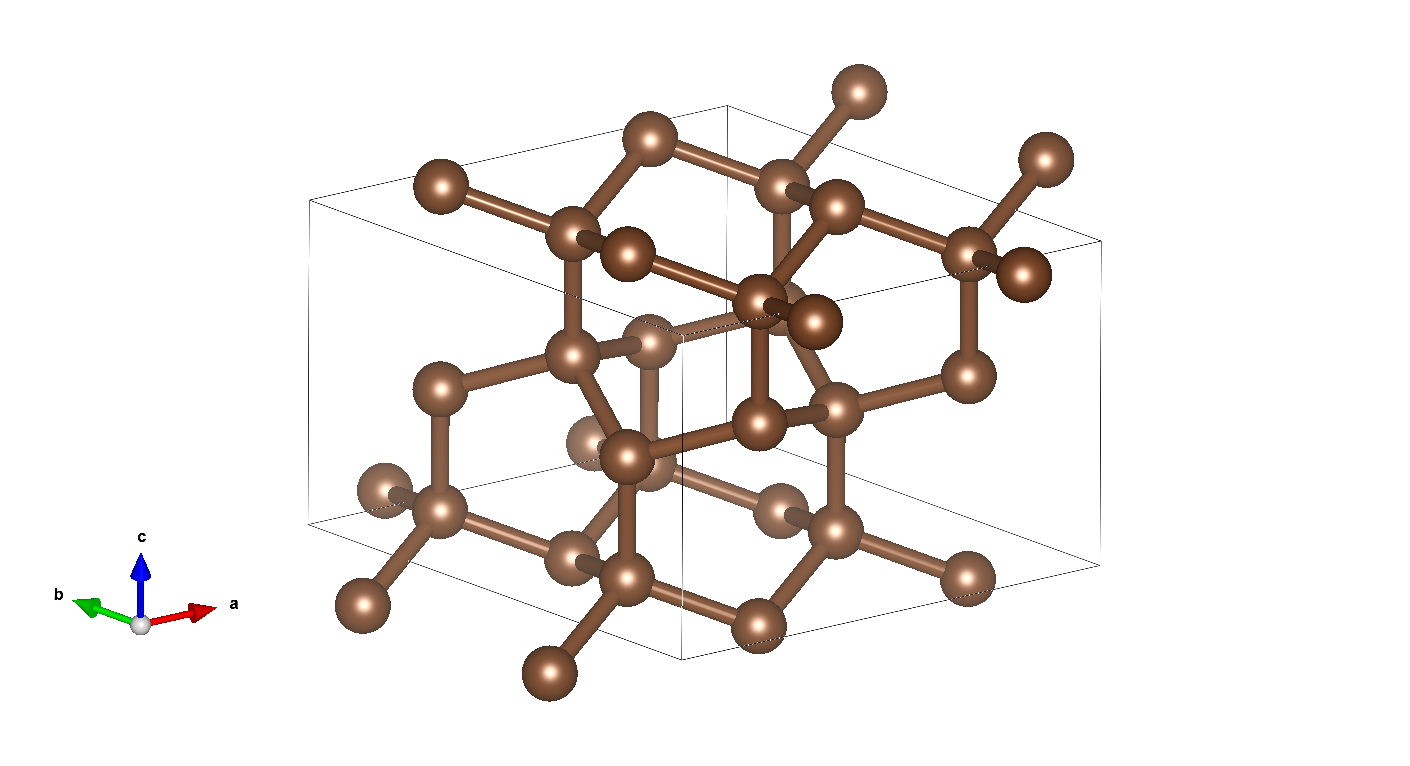
\includegraphics[width=0.5\textwidth, trim=0 0 27em 0,clip]{images/poscar_hex_16_birdseye.png}
  \end{center}
\end{frame}

\begin{frame}{Defected hexagonal diamond}
  \begin{center}
    \begin{tabular}{cr}
      Cubic diamond   & 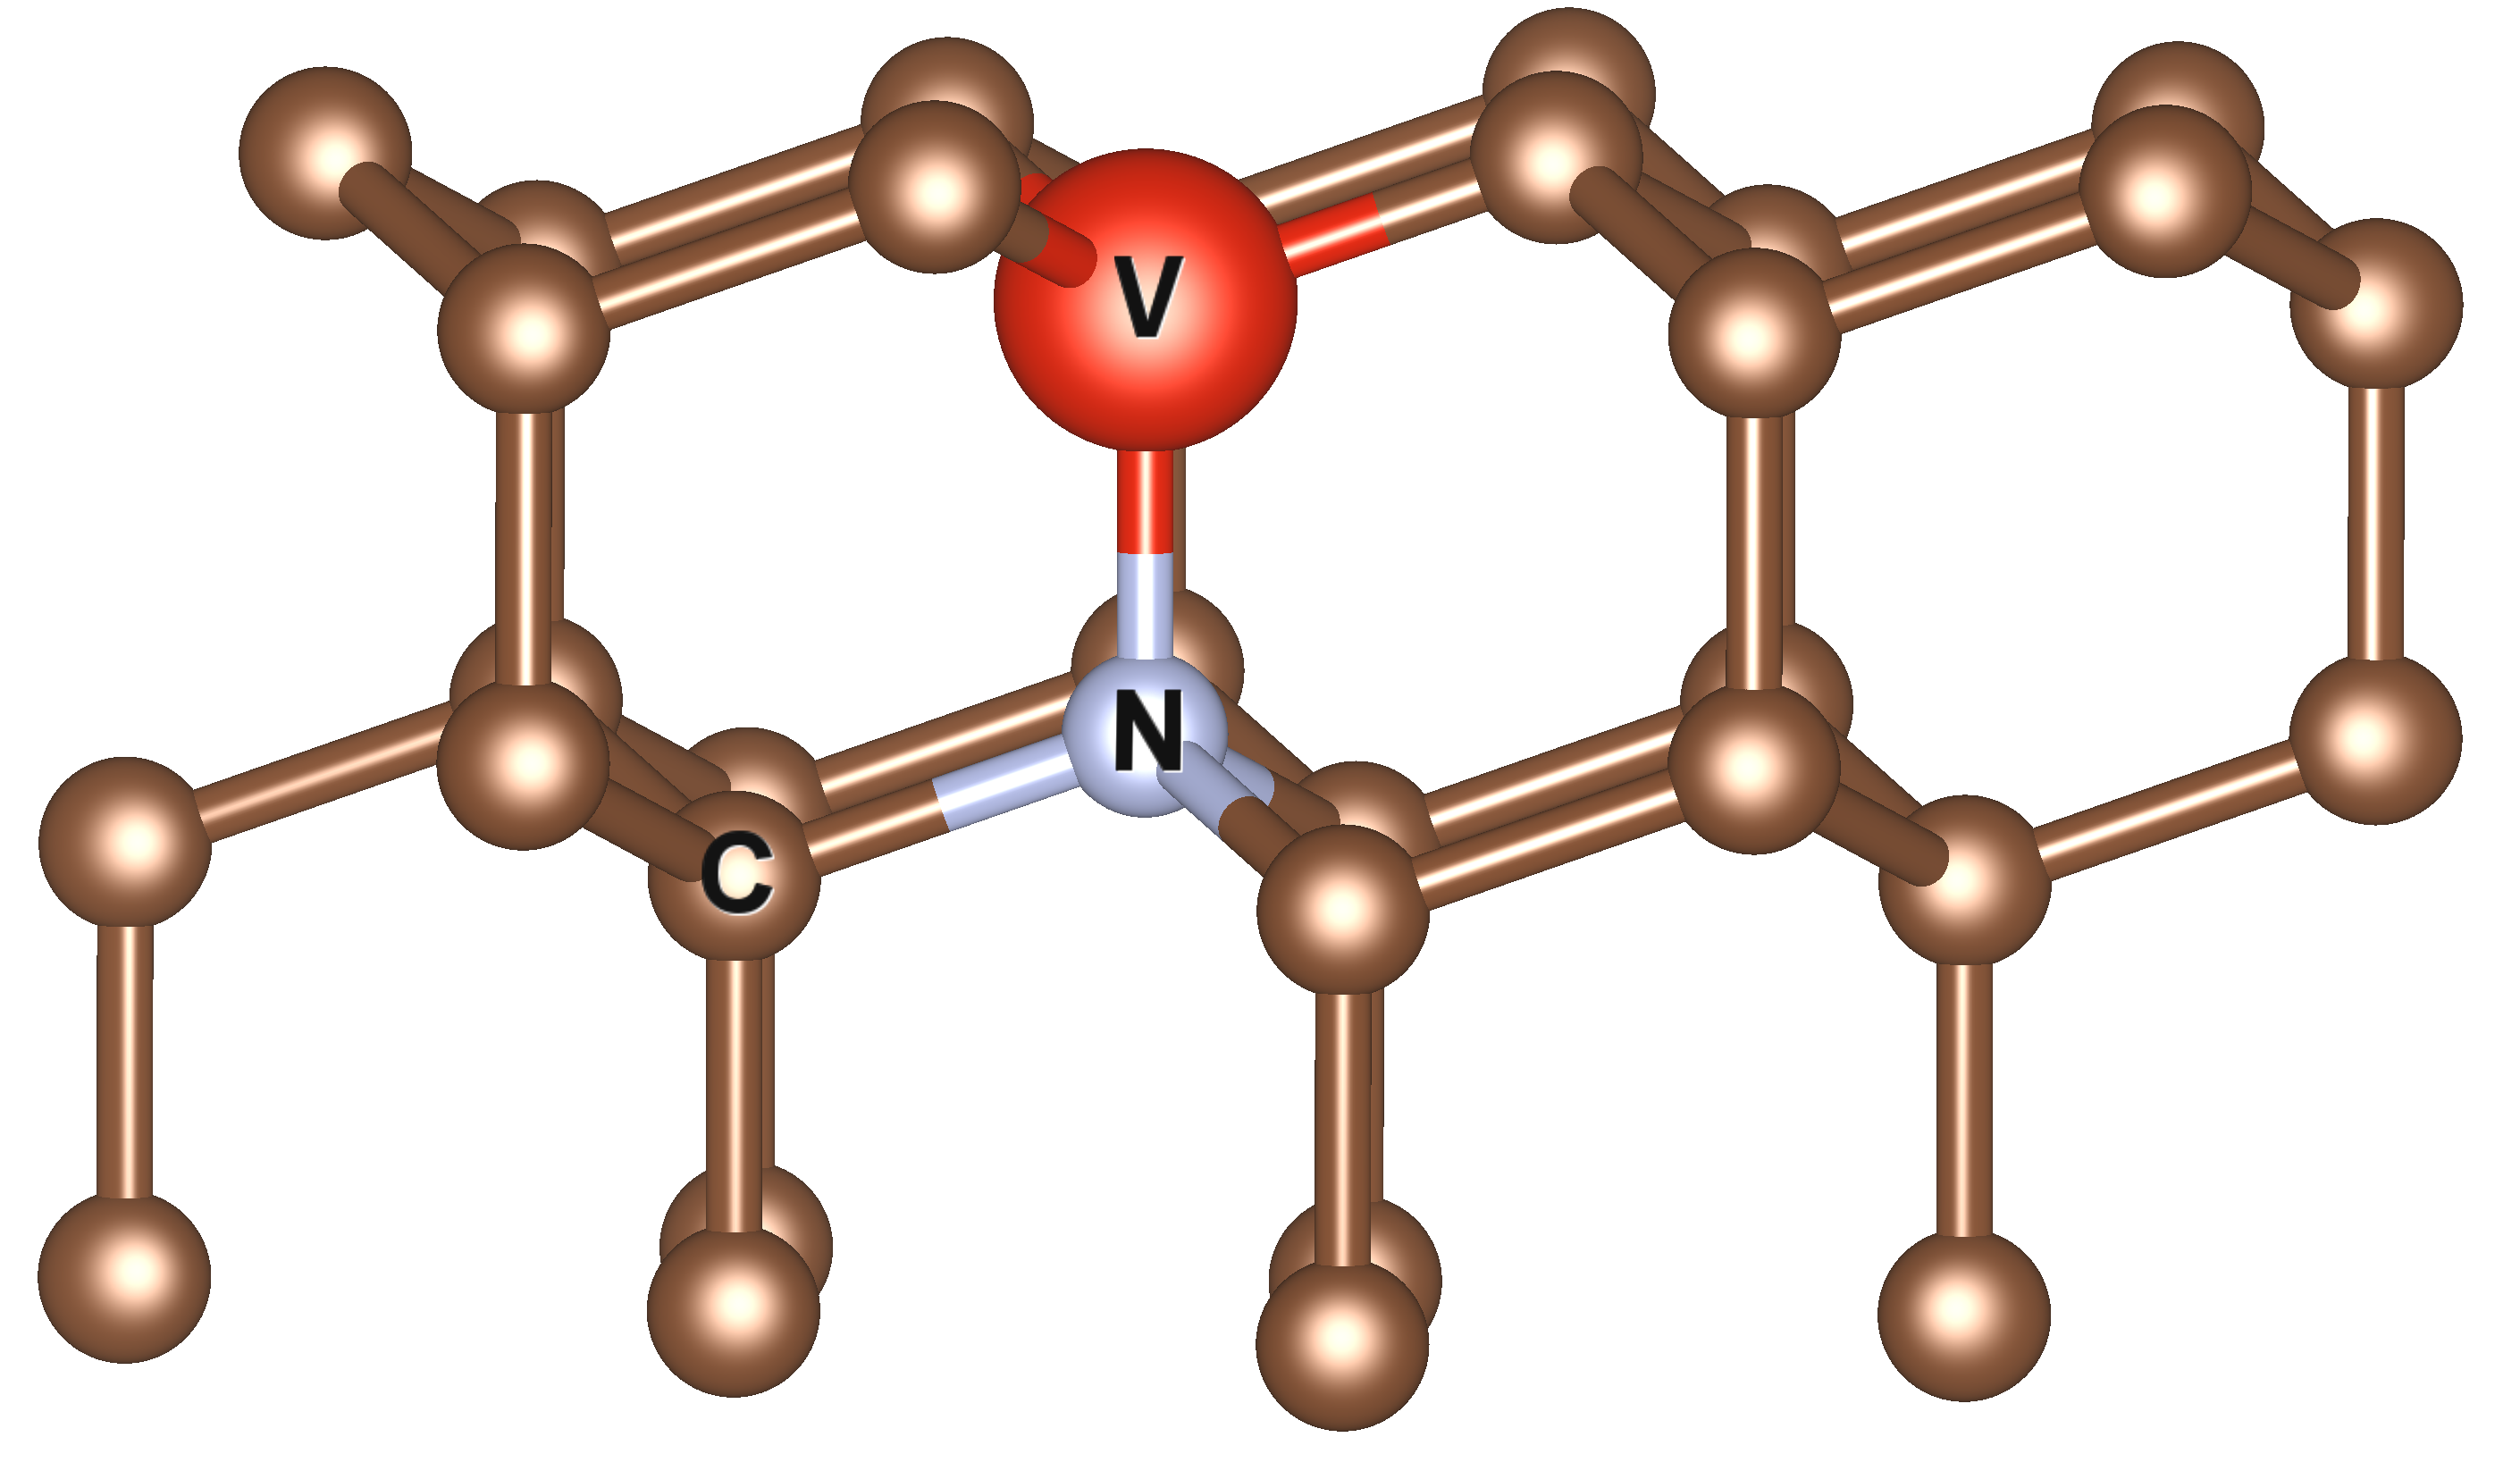
\includegraphics[width=0.4\textwidth]{images/POSCAR_16_view.png}\\
      Hexagonal $ x $-type &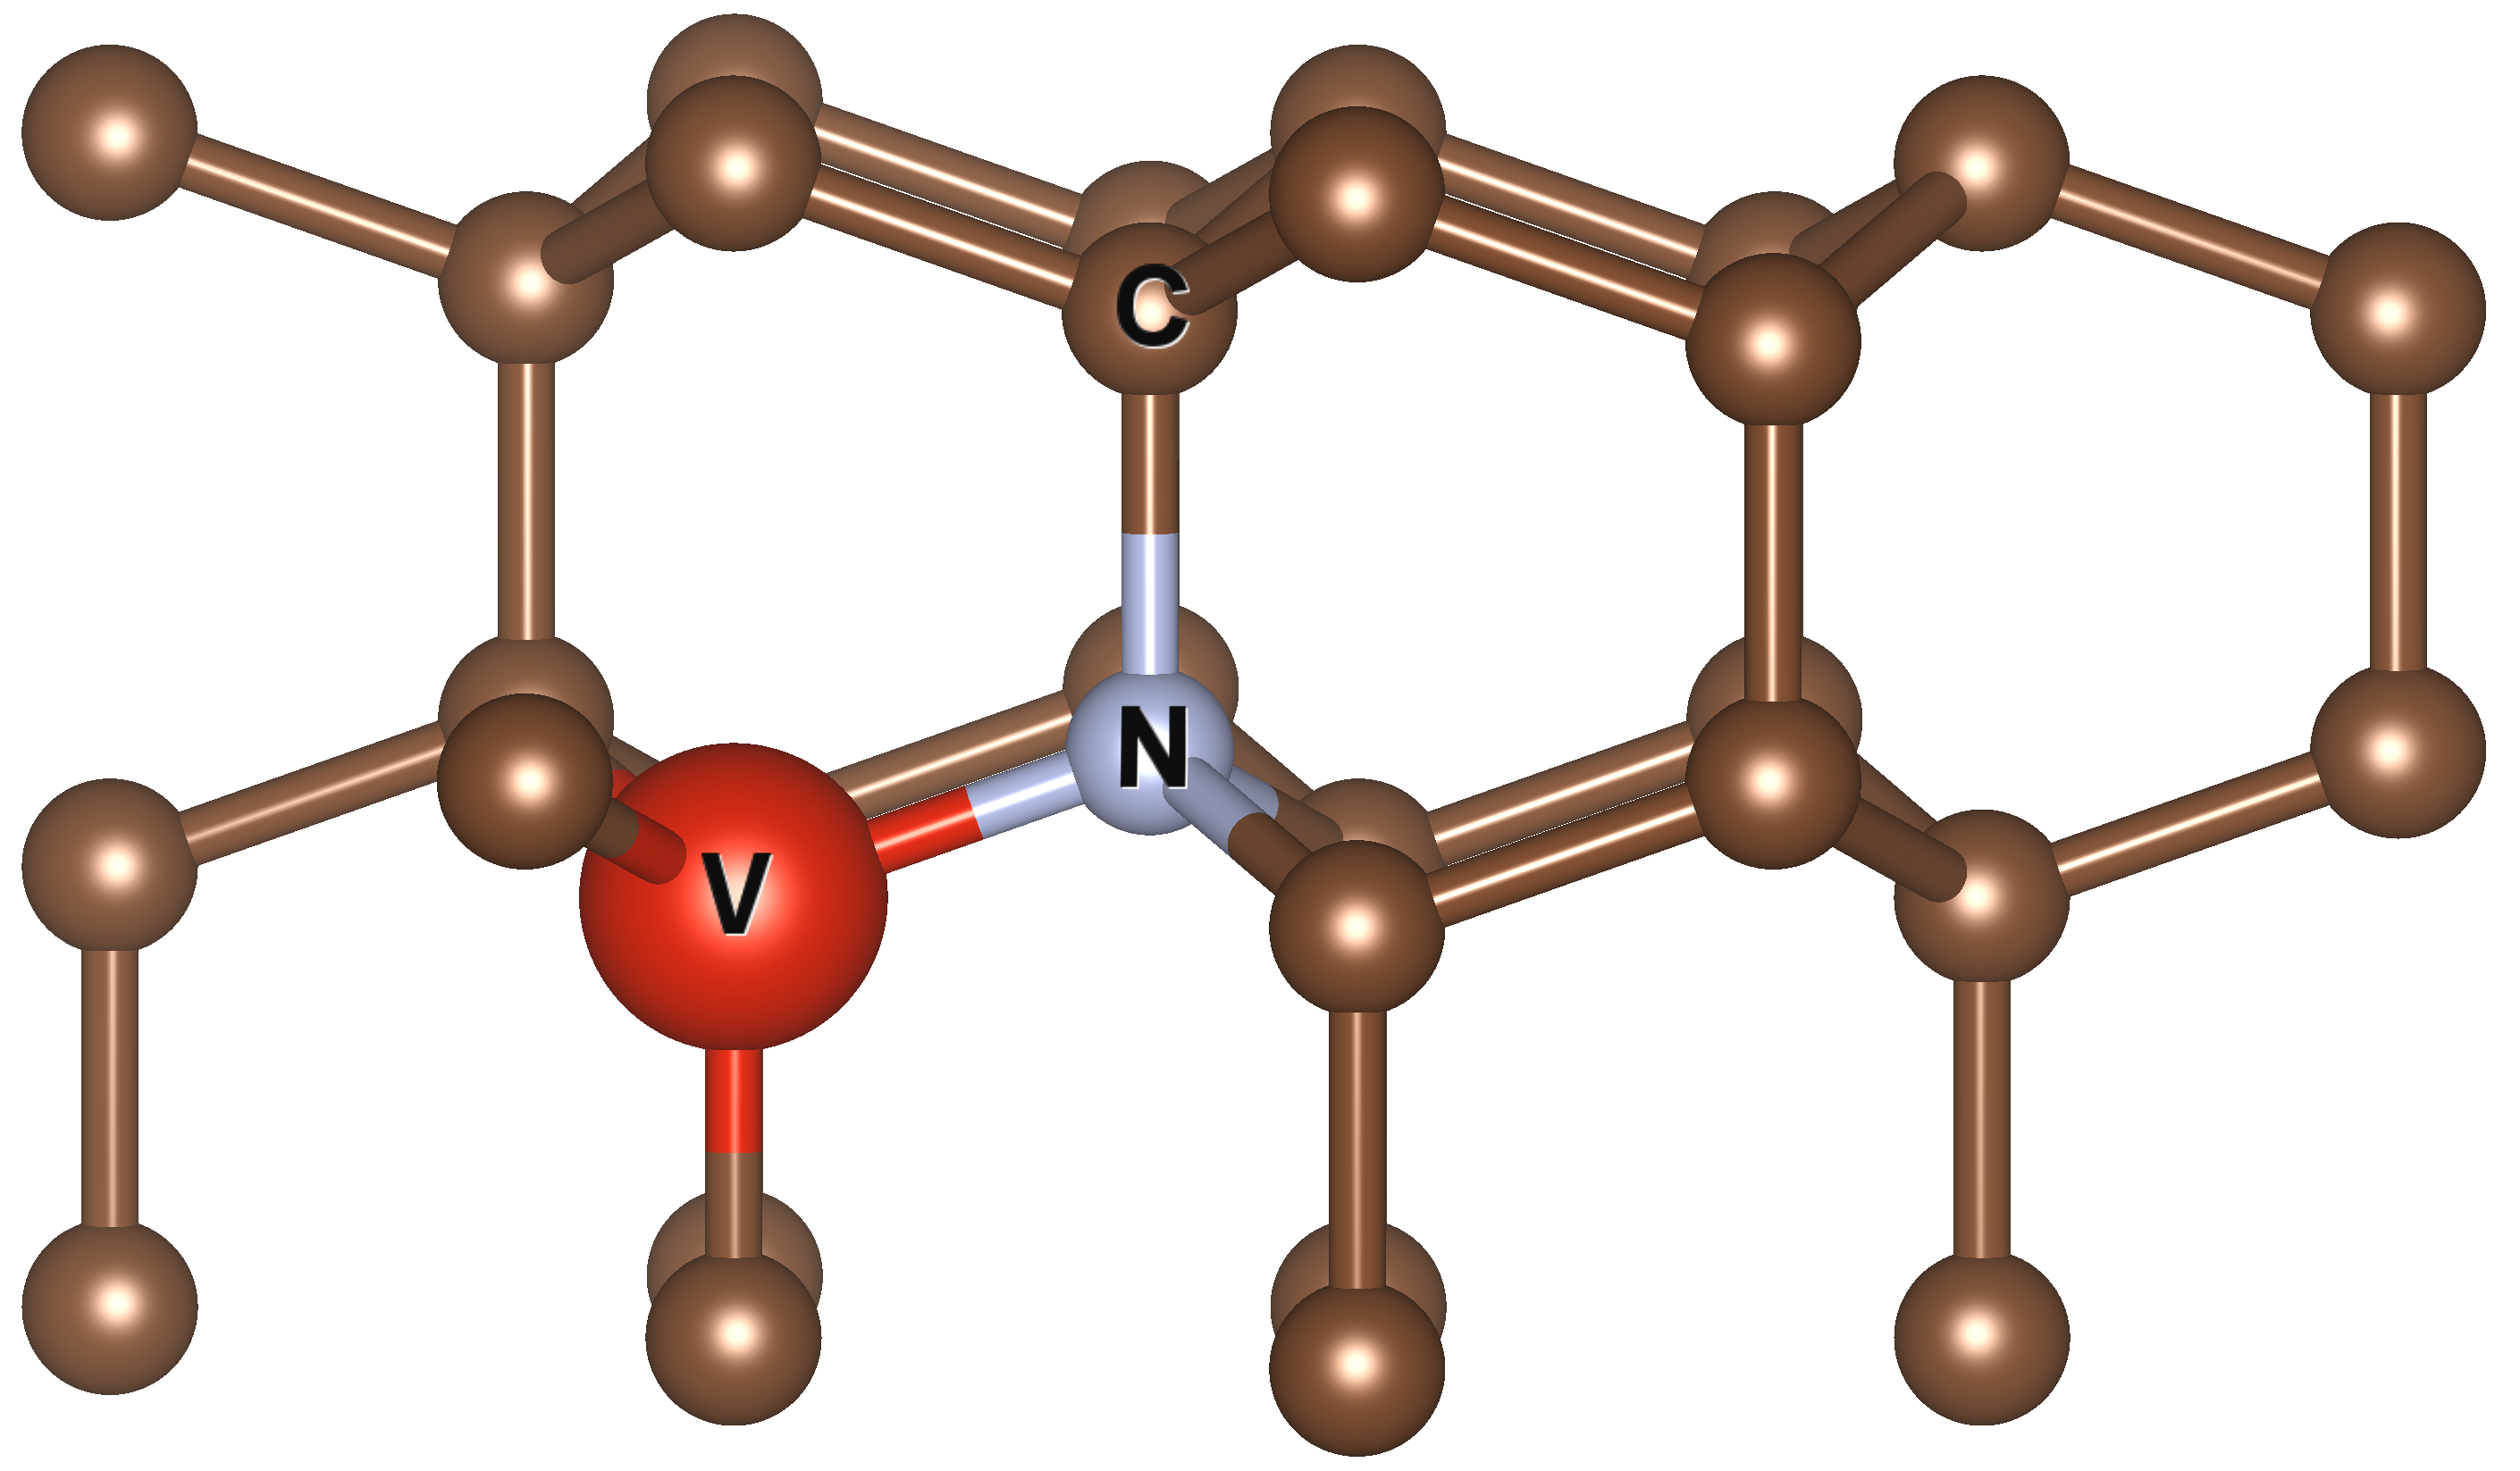
\includegraphics[width=0.4\textwidth]{images/POSCAR_16_x_view.png}\\
      Hexagonal $ z $-type & 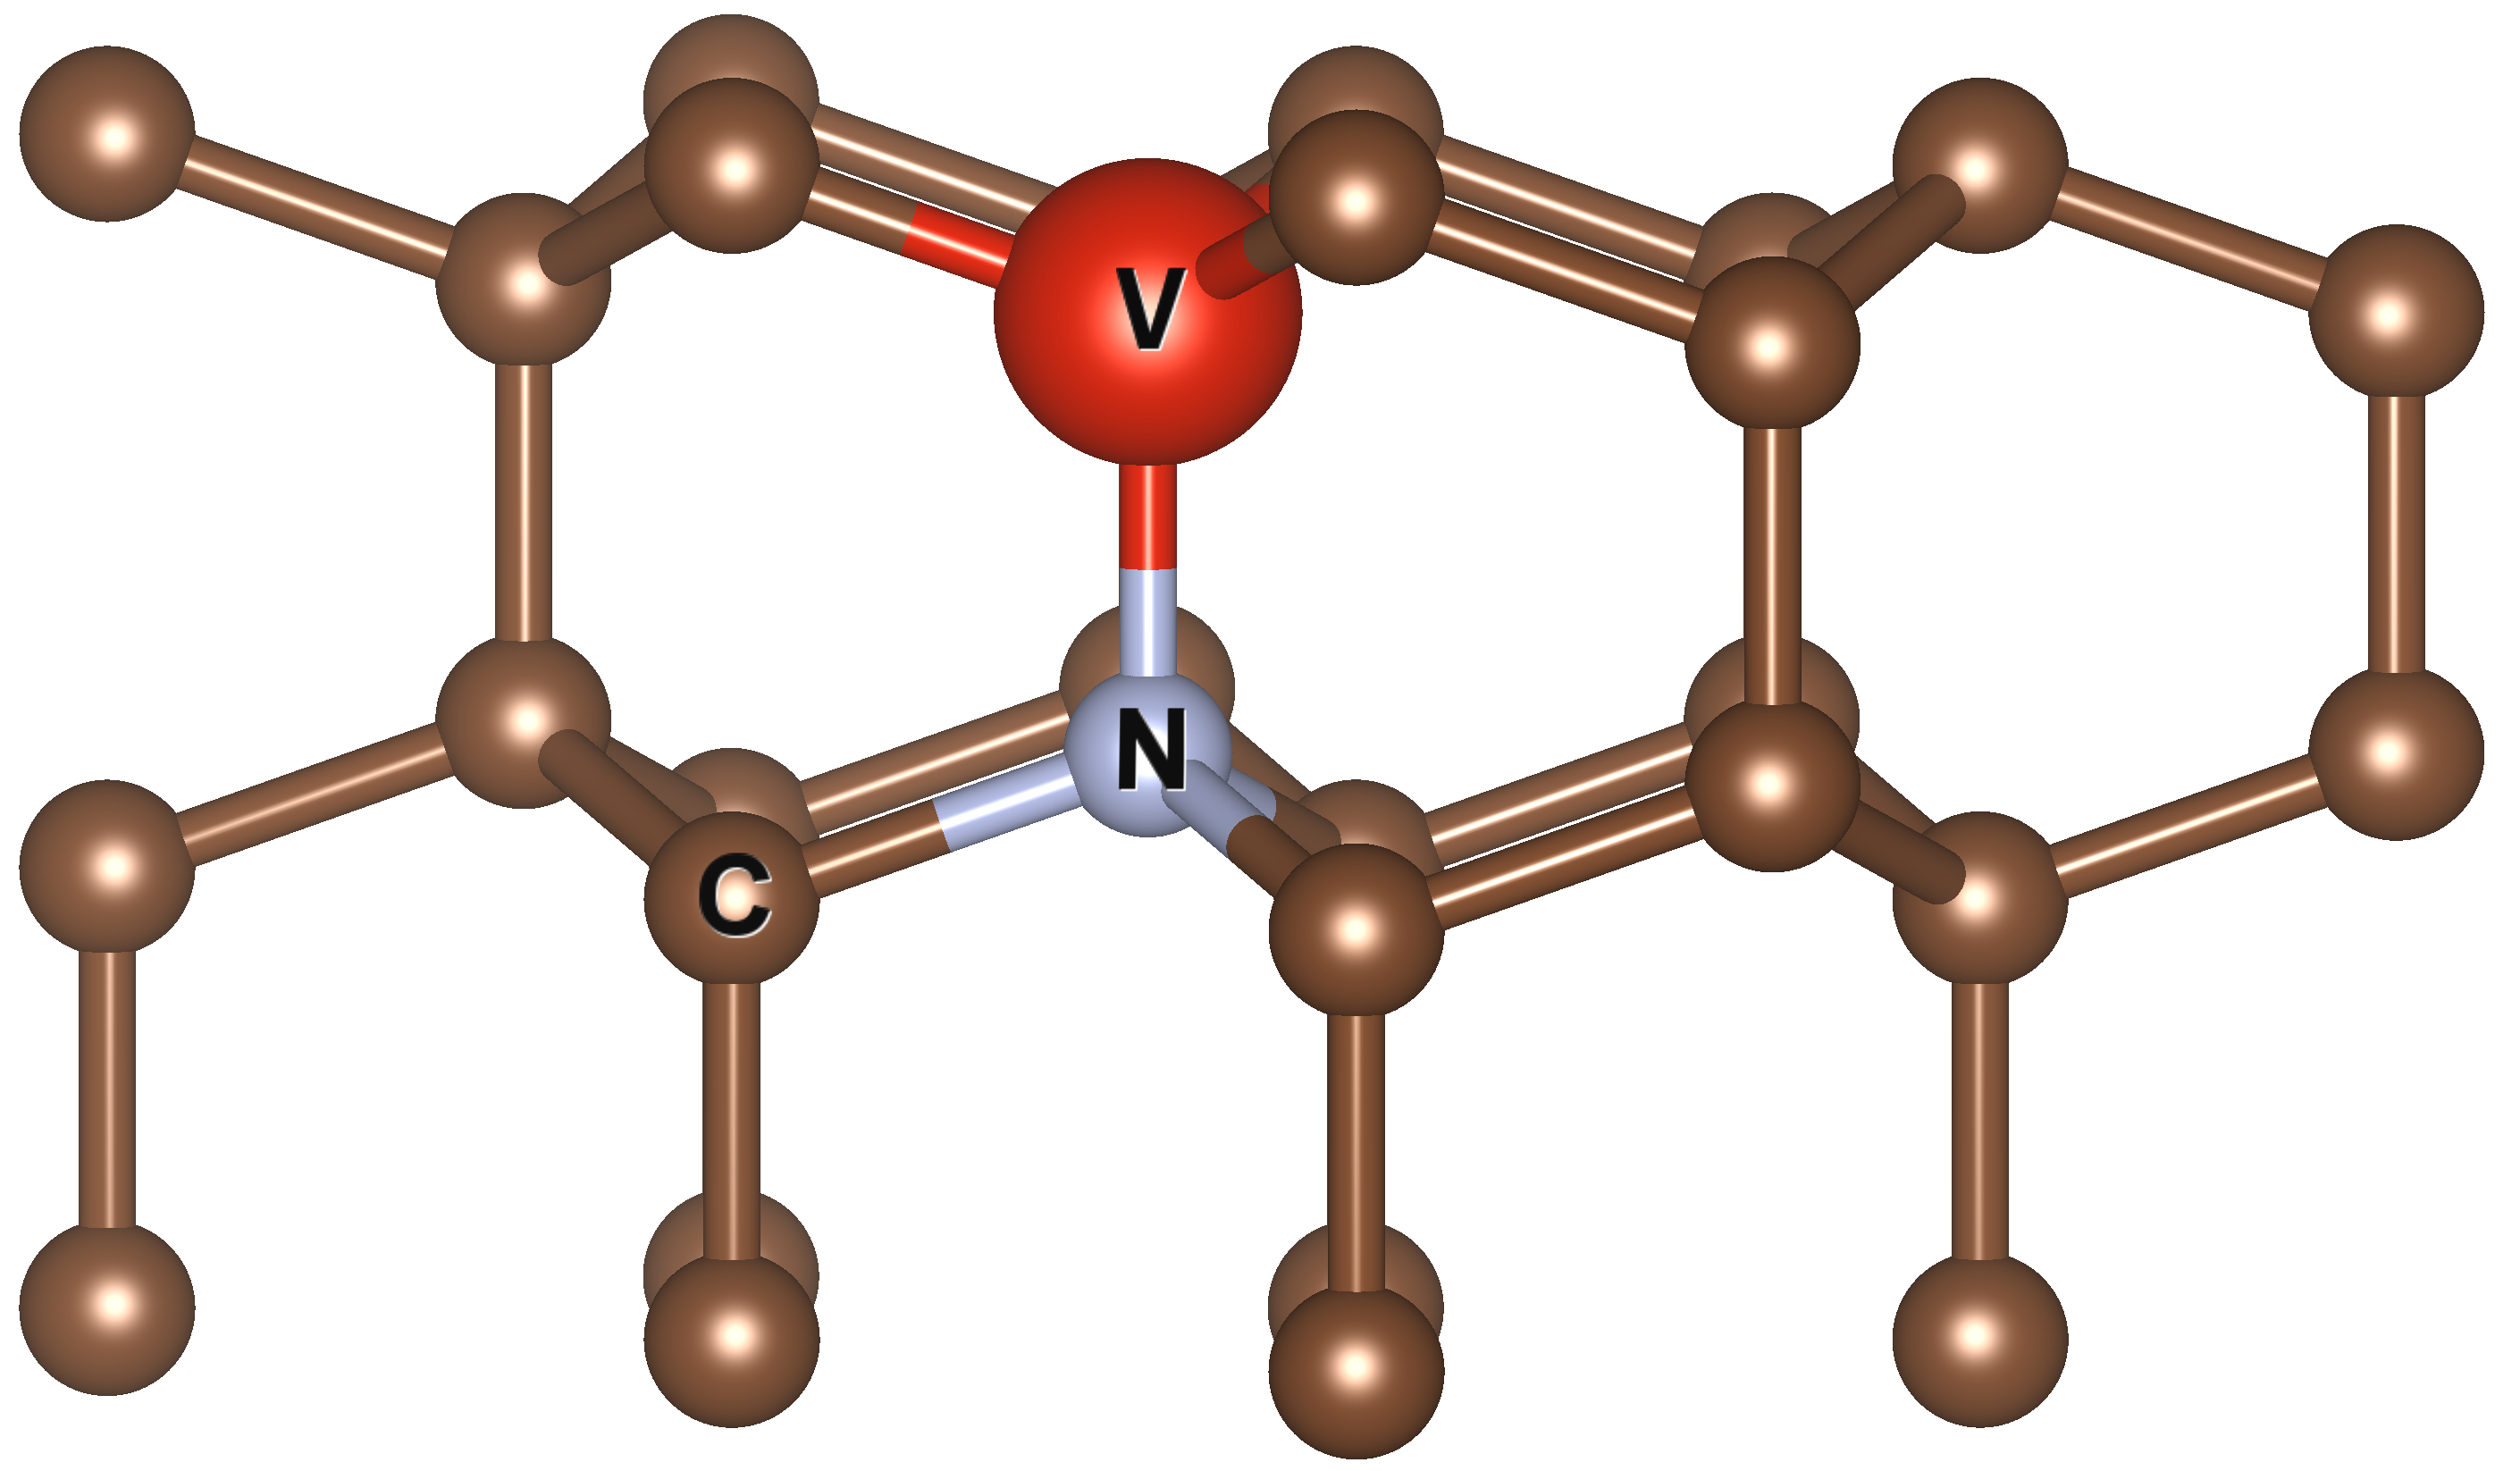
\includegraphics[width=0.4\textwidth]{images/POSCAR_16_z_view.png}
    \end{tabular}
  \end{center}
\end{frame}



%\begin{frame}{Split vacancies: $ \mathsf{SiV}^{-} $  }
  %\def\splitTrim{6}
  %\def\splitTrimVertical{2}
  %\begin{columns}
    %\begin{column}{0.5\textwidth}
      %\includegraphics[width=\textwidth, keepaspectratio,trim=\splitTrim cm \splitTrimVertical cm \splitTrim cm \splitTrimVertical cm,clip]{images/poscar__si_minux_definitiv_1.pdf}
    %\end{column}
    %\begin{column}{0.5\textwidth}
      %\includegraphics[width=\textwidth, keepaspectratio,trim=\splitTrim cm \splitTrimVertical cm \splitTrim cm \splitTrimVertical cm,clip]{images/contcar__si_minux_definitiv_1_cartesian.pdf}
    %\end{column}
  %\end{columns}
%\end{frame}


\section{Results} %{{{1

\begin{frame}{ $ \mathsf{NV}^{-} $: Ground state $ ^3A_{2} $ }
  \begin{center}
    \begin{columns}
      \begin{column}{0.3\textwidth}
        \includegraphics[height=1\textheight]{images/lumos/N_minus_cubic_128_dmatrix_encut_lumos.pdf}
      \end{column}
      \begin{column}{0.3\textwidth}
        \includegraphics[height=1\textheight]{images/lumos/N_minus_hexagonal_z_128_dmatrix_encut_lumos.pdf}
      \end{column}
      \begin{column}{0.3\textwidth}
        \includegraphics[height=1\textheight]{images/lumos/N_minus_hexagonal_x_128_dmatrix_encut_lumos.pdf}
      \end{column}
    \end{columns}
  \end{center}
\end{frame}

\begin{frame}{ $ \mathsf{NV}^{-} $: Excited state $ ^3E $ }
  \begin{center}
    \begin{columns}
      \begin{column}{0.3\textwidth}
        \includegraphics[height=1\textheight]{images/lumos/excited/N_minus_cubic_128_B_OUTCAR.pdf}
      \end{column}
      \begin{column}{0.3\textwidth}
        \includegraphics[height=1\textheight]{images/lumos/excited/N_minus_hexagonal_z_128_B_OUTCAR.pdf}
      \end{column}
      \begin{column}{0.3\textwidth}
        \includegraphics[height=1\textheight]{images/lumos/excited/N_minus_hexagonal_x_128_B_OUTCAR.pdf}
      \end{column}
    \end{columns}
  \end{center}
\end{frame}

\begin{frame}{$ \mathsf{NV}^{-} $: ZFS }
  \begin{itemize}
    \item
      \textit{Cubic diamond, convergence and comparison with the experimental result.}
  \end{itemize}
  \includegraphics[width=1.0\textwidth, trim=0 0 0em 0,clip]{images/zfs_cubic/plot_cubic.pdf}
\end{frame}

\begin{frame}{$ \mathsf{NV}^{*} $: ZFS cubic ($ \mathsf{NV}^{*}_{c} $), Hexagonal $ x,z $ ($ \mathsf{NV}_{x,z}^{*} $)   }
  \includegraphics[width=1.0\textwidth, trim=0 0 0em 0,clip]{images/splitting_comparison/dmatrix_encut/N_all.pdf}
\end{frame}









\begin{frame}{ $ \mathsf{NV}^{-} $: Vibronic scheme (PBE + 128 atomic cell)}

  \begin{center}
    \includegraphics<1>[width=.5\textwidth]{images/vibronic.pdf}
  \end{center}

  \only<2>{
    \begin{columns}
      \begin{column}{0.3333\textwidth}
        \centering
        \textit{Cubic }
        \includegraphics[width=1\textwidth, trim=0 0 0em 0,clip]{images/abcd/abcd_128_zinc.pdf}
      \end{column}
      \begin{column}{0.3333\textwidth}
        \centering
        \textit{Hexagonal $ x $ }
        \includegraphics[width=1\textwidth, trim=0 0 0em 0,clip]{images/abcd/abcd_128_z.pdf}
      \end{column}
      \begin{column}{0.3333\textwidth}
        \centering
        \textit{Hexagonal $ z $ }
        \includegraphics[width=1\textwidth, trim=0 0 0em 0,clip]{images/abcd/abcd_128_x.pdf}
      \end{column}
    \end{columns}
  }
  \only<3->{
    \begin{columns}
      \begin{column}{0.3333\textwidth}
        \centering
        \textit{Cubic }
        \includegraphics[width=1\textwidth, trim=0 0 0em 0,clip]{images/abcd/abcd_128_zinc.pdf}
      \end{column}
      \begin{column}{0.3333\textwidth}
        \begin{center}
          \small
          \begin{tabular}{lc}
            \hline
            \multicolumn{2}{c}{Experimental data}\\
            \hline
            ZPL & 1.945\\
            \hline
            $ ^3A_2 \to ^3E^{*} $  & 2.180\\
            \hline
            $ S $  & 0.235\\
            \hline
            $  ^3E \to ^3A_2^{*} $ & 1.760\\
            \hline
            $ AS $  & 0.185\\
            \hline
          \end{tabular}
        \end{center}
      \end{column}
      \begin{column}{0.3333\textwidth}
        \begin{center}
          \small
          \begin{tabular}{lc}
            \hline
            \multicolumn{2}{c}{Calculations}\\
            \hline
            ZPL & 1.693\\
            \hline
            $ ^3A_2 \to ^3E^{*} $  & 1.842\\
            \hline
            $ S $  & 0.150\\
            \hline
            $  ^3E \to ^3A_2^{*} $  & 1.549\\
            \hline
            $ AS $  & 0.144\\
            \hline
          \end{tabular}
        \end{center}
      \end{column}
    \end{columns}
    }
  \end{frame}

\begin{frame}{Expanding the defect}
  \begin{center}
    \includegraphics[height=.9\textheight]{images/elements.pdf}
  \end{center}
\end{frame}

\begin{frame}{Expanding the defect}
  \begin{center}
    \includegraphics[height=0.9\textheight]{images/elements_vacancies.pdf}
  \end{center}
\end{frame}

\begin{frame}{ZFS map}
  \begin{center}
    \includegraphics[width=1\textwidth]{images/splitting_comparison/dmatrix_encut/all.pdf}
  \end{center}
\end{frame}


  
\begin{frame}{Ground state example: $ \mathsf{GeV}^{-} $ }
  \begin{center}
    \begin{columns}
      \begin{column}{0.3\textwidth}
        \includegraphics[height=1\textheight]{images/lumos/Ge_minus_cubic_128_dmatrix_encut_lumos.pdf}
      \end{column}
      \begin{column}{0.3\textwidth}
        \includegraphics[height=1\textheight]{images/lumos/Ge_minus_hexagonal_z_128_dmatrix_encut_lumos.pdf}
      \end{column}
      \begin{column}{0.3\textwidth}
        \includegraphics[height=1\textheight]{images/lumos/Ge_minus_hexagonal_x_128_dmatrix_encut_lumos.pdf}
      \end{column}
    \end{columns}
  \end{center}
\end{frame}



\section{Summary and outlook} %{{{1




\begin{frame}{Where we are, and where to go next\ldots}
  \begin{itemize}
    \item Structural properties
    \item ZPL calculation.
    \item ZFS tensor calculation.
    \item \textbf{Beyond the Ground state:}\\
      Using DMRG (\textit{Density Matrix Renormalization Group}) for excited state calculations
  \end{itemize}
\end{frame}


\begin{frame}{Using DMRG for excited state calculations}
  \begin{columns}
    \begin{column}{0.5\textwidth}
      \begin{itemize}
        \item $ \mathsf{XV}^{q} $ as molecules.
        \item Localized states as isolated.
        \item Issues like charge transfer, charge corrections.
      \end{itemize}
    \end{column}
    \begin{column}{0.5\textwidth}
      \centering
      \textit{ $ \mathsf{NV}^{+} $ }
      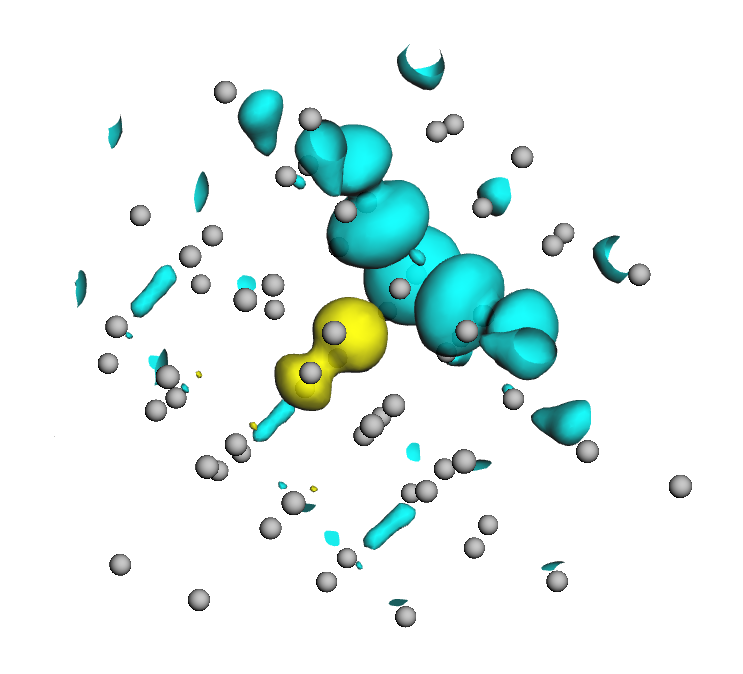
\includegraphics[clip, trim=2cm 0 2cm 0, width=1.0\textwidth]{images/nv_plus_orbitals_example.png}
    \end{column}
  \end{columns}
\end{frame}


\plain{Thank you!}





\end{document}



\end{document}


% vim: spell fdm=marker :
%vim-run: pdflatex %; make all
%vim-run: make all
